\documentclass[11pt,a4paper]{article}

% Packages
\usepackage[utf8]{inputenc}
\usepackage[T1]{fontenc}
\usepackage{amsmath,amssymb,amsthm}
\usepackage{mathtools}
\usepackage{geometry}
\usepackage{hyperref}
\usepackage{cleveref}
\usepackage{enumitem}
\usepackage{graphicx}
\usepackage{tikz}
\usepackage{pgfplots}
\pgfplotsset{compat=1.18}
\usepackage{booktabs}

\geometry{margin=1in}

% Theorem environments
\newtheorem{theorem}{Theorem}[section]
\newtheorem{lemma}[theorem]{Lemma}
\newtheorem{proposition}[theorem]{Proposition}
\newtheorem{corollary}[theorem]{Corollary}
\theoremstyle{definition}
\newtheorem{definition}[theorem]{Definition}
\newtheorem{assumption}[theorem]{Assumption}
\theoremstyle{remark}
\newtheorem{remark}[theorem]{Remark}

% Macros
\newcommand{\R}{\mathbb{R}}
\newcommand{\E}{\mathbb{E}}
\newcommand{\Prob}{\mathbb{P}}
\newcommand{\Cov}{\mathrm{Cov}}
\newcommand{\tr}{\mathrm{tr}}
\newcommand{\op}{\mathrm{op}}
\newcommand{\supp}{\mathrm{supp}}
\DeclareMathOperator{\sgn}{sgn}
\DeclareMathOperator*{\argmin}{arg\,min}
\DeclareMathOperator*{\argmax}{arg\,max}

\title{Spectral Phase Transitions in the Loss Landscape\\of Finite-Width Neural Networks}
\author{Jacob Crainic}
\date{February 2026}

\begin{document}
\maketitle

\begin{abstract}
A central puzzle in deep learning theory is why gradient descent reliably finds good solutions despite the extreme non-convexity of neural network loss landscapes, particularly in the moderately overparameterized regime where existing theoretical guarantees require polynomial width scaling far exceeding practical network sizes.
We study the critical-point structure of the empirical risk landscape for two-layer
neural networks with ReLU activations, trained on $n$ data points in $\R^d$ with $m$ hidden
neurons. Our main result establishes a sharp phase transition in the Hessian spectrum
at critical points: when the width-to-sample ratio $\gamma = m/n$ crosses a critical threshold
$\gamma_\star$ that depends on the spectral distribution of the data covariance, all spurious local
minima are eliminated with high probability. Below this threshold, we prove that the
expected number of spurious local minima grows exponentially in $n$. The critical ratio
$\gamma_\star$ is characterized as the unique solution to a fixed-point equation involving the
Stieltjes transform of the Marchenko--Pastur law composed with the data spectrum.
For isotropic data ($\Sigma = I_d$), the critical ratio takes the explicit form
$\gamma_\star(\delta) = \frac{4}{2 + 3\delta}$, where $\delta = d/n$.
We further show that at the transition, the Hessian at near-critical points exhibits a
spectral gap collapse: the smallest non-zero eigenvalue vanishes as $|\gamma - \gamma_\star|^{1/2}$, yielding
a universal square-root scaling law. Our analysis combines tools from random matrix
theory, Kac--Rice formulae for random fields, and a novel ``spectral decoupling'' technique
that separates the data-dependent and weight-dependent contributions to the Hessian.
\end{abstract}

\tableofcontents

%% ============================================================
\section{Introduction}
%% ============================================================

A central question in the theory of deep learning is: why does gradient descent find good
solutions despite the non-convexity of the loss landscape? The empirical risk of a neural
network is a highly non-convex function of its parameters, and classical optimization theory
predicts that gradient-based methods should become trapped in poor local minima. Yet in
practice, this rarely occurs.

A growing body of work \cite{choromanska2015,kawaguchi2016,safran2018,venturi2019} has provided partial explanations by studying
the geometry of the loss surface. The overparameterized regime---where the number of
parameters exceeds the number of data points---has received particular attention, with
results showing that all local minima become global in sufficiently wide networks \cite{du2019,allenzhu2019}.
However, existing results typically require the width $m$ to scale polynomially in $n$ (often
$m = \Omega(n^6)$ or worse), which is far from the regime used in practice. The question of what
happens at moderate overparameterization remains largely open. In this paper, we give a
precise answer for two-layer ReLU networks.

\subsection{Main contributions}

\begin{enumerate}[label=(\roman*)]
  \item \textbf{Sharp threshold.} We identify a critical width-to-sample ratio $\gamma_\star$ (depending on the
  data covariance spectrum) such that for $\gamma > \gamma_\star$, all local minima of the empirical risk
  are global with probability $1 - e^{-\Omega(n)}$, and for $\gamma < \gamma_\star$, there exist exponentially many
  spurious local minima (Theorem~\ref{thm:phase-transition}).

  \item \textbf{Spectral characterization.} We give an explicit fixed-point equation for $\gamma_\star$ in terms
  of the Stieltjes transform of the limiting spectral distribution of the data Gram matrix
  (Theorem~\ref{thm:critical-ratio}).

  \item \textbf{Universal scaling at the transition.} We prove that the spectral gap of the Hessian
  at critical points scales as $|\gamma - \gamma_\star|^{1/2}$ near the transition, establishing universality of
  the critical exponent (Theorem~\ref{thm:scaling}).

  \item \textbf{Spectral decoupling technique.} We introduce a decomposition of the Hessian
  at critical points into a ``data block'' and a ``weight block'' coupled through a rank-deficient
  interaction term (Section~\ref{sec:decoupling}), which may be of independent interest.
\end{enumerate}

\subsection{Related work}

\paragraph{Loss landscape of neural networks.}
Choromanska et al.\ \cite{choromanska2015} drew an analogy between
neural network loss surfaces and spin glass models. Kawaguchi \cite{kawaguchi2016} showed that for linear
networks, every local minimum is global. Safran and Shamir \cite{safran2018} demonstrated the existence
of spurious local minima for two-layer ReLU networks but in the underparameterized regime.
Our work precisely locates the transition between these regimes.

\paragraph{Overparameterization and global convergence.}
Du et al.\ \cite{du2019}, Allen-Zhu et al.\ \cite{allenzhu2019},
and Zou et al.\ \cite{zou2020} proved that gradient descent converges to global minima when $m$ is
polynomially large in $n$. The Neural Tangent Kernel (NTK) framework \cite{jacot2018} provides a
complementary view via linearization. Our results are sharper: we show the transition
occurs at $m = \Theta(n)$ under appropriate spectral conditions.

\paragraph{Random matrix theory in ML.}
Pennington and Worah \cite{pennington2017} and Louart et al.\ \cite{louart2018}
applied random matrix theory to understand neural network Jacobians and kernel matrices.
Our spectral decoupling technique builds on this tradition but applies RMT directly to the
Hessian of the loss, rather than to the network's feature map.

%% ============================================================
\section{Problem Setup}
%% ============================================================

\subsection{Network architecture and loss}

Consider a two-layer neural network $f_\theta : \R^d \to \R$ with $m$ hidden neurons:
\begin{equation}\label{eq:network}
  f_\theta(x) = \frac{1}{\sqrt{m}} \sum_{j=1}^{m} a_j\, \sigma(w_j^\top x),
\end{equation}
where $\sigma(t) = \max(0,t)$ is the ReLU activation, $w_j \in \R^d$ are the first-layer weights,
$a_j \in \R$ are the second-layer weights, and $\theta = (W, a)$ with
$W = [w_1, \ldots, w_m]^\top \in \R^{m \times d}$ and $a = (a_1, \ldots, a_m)^\top \in \R^m$.
The $1/\sqrt{m}$ scaling is the mean-field (``NTK'') parameterization.

Given training data $\{(x_i, y_i)\}_{i=1}^n$ with $x_i \in \R^d$ and $y_i \in \R$, the empirical risk is:
\begin{equation}\label{eq:loss}
  L(\theta) = \frac{1}{2n} \sum_{i=1}^{n} \bigl(f_\theta(x_i) - y_i\bigr)^2.
\end{equation}

\subsection{Data model}

\begin{assumption}[Data distribution]\label{ass:data}
  The data points $x_1, \ldots, x_n$ are i.i.d.\ draws from $\mathcal{N}(0, \Sigma)$ where
  $\Sigma \in \R^{d \times d}$ is positive definite. We work in the proportional regime where
  $d, n, m \to \infty$ with:
  \[
    d/n \to \delta \in (0,\infty), \qquad m/n \to \gamma \in (0,\infty).
  \]
  The empirical spectral distribution of $\Sigma$ converges weakly to a compactly supported
  probability measure $\mu_\Sigma$ on $(0,\infty)$.
\end{assumption}

\begin{assumption}[Labels]\label{ass:labels}
  The labels are generated by a ``teacher'' network:
  $y_i = f_{\theta^*}(x_i) + \varepsilon_i$ where $\theta^*$ has $m^*$ hidden neurons with
  $m^*/n \to \gamma^* \le \gamma$, and $\varepsilon_i \sim \mathcal{N}(0, \sigma_\varepsilon^2)$ i.i.d.
\end{assumption}

\subsection{The Hessian structure}

At any point $\theta$, define the residual vector $r(\theta) \in \R^n$ with
$r_i(\theta) = f_\theta(x_i) - y_i$, and the Jacobian $J(\theta) \in \R^{n \times p}$ with
$p = m(d+1)$ and $J_{ij} = \partial f_\theta(x_i)/\partial\theta_j$. Due to the ReLU
non-differentiability, $J$ is defined almost everywhere. The Hessian of $L$ decomposes as:
\begin{equation}\label{eq:hessian-decomp}
  \nabla^2 L(\theta) = \frac{1}{n} J(\theta)^\top J(\theta)
    + \frac{1}{n} \sum_{i=1}^{n} r_i(\theta)\, \nabla^2 f_\theta(x_i).
\end{equation}
At a critical point where $\nabla L(\theta) = 0$, the first (Gauss--Newton) term
$\frac{1}{n} J^\top J$ is always positive semidefinite, while the second (residual) term can
have negative eigenvalues. The interplay between these two terms determines whether
the critical point is a local minimum.

%% ============================================================
\section{The Spectral Decoupling}\label{sec:decoupling}
%% ============================================================

Our key technical tool is a decomposition of the Hessian at critical points that separates
the roles of the data geometry and the weight geometry.

\begin{definition}[Activation pattern]\label{def:activation}
  For weight matrix $W \in \R^{m \times d}$, define the activation pattern matrix
  $D(W, X) \in \R^{nm \times nm}$ as the block-diagonal matrix with diagonal blocks
  $D_{ij} = \mathbf{1}[w_j^\top x_i > 0]$ for $i \in [n]$, $j \in [m]$.
\end{definition}

\begin{definition}[Data-weight interaction matrix]\label{def:kernel}
  Define the effective kernel matrix $K_\theta \in \R^{n \times n}$ by:
  \begin{equation}\label{eq:kernel}
    (K_\theta)_{ik} = \frac{1}{m} \sum_{j=1}^{m} a_j^2\, \mathbf{1}[w_j^\top x_i > 0]\,
    \mathbf{1}[w_j^\top x_k > 0]\, \frac{x_i^\top x_k}{\|w_j\|^2} \cdot
    \frac{w_j^\top x_i\, w_j^\top x_k}{\|w_j\|^2}.
  \end{equation}
  (Note: the kernel $K_\theta$ resembles the neural tangent kernel restricted to the first
  layer, but with the additional gating from activation patterns.)
\end{definition}

\begin{proposition}[Hessian block decomposition]\label{prop:block}
  At any critical point $\theta_c$ of $L$, the Hessian in \eqref{eq:hessian-decomp} can be
  written in the block form with respect to the partition $\theta = (W, a)$:
  \begin{equation}\label{eq:block}
    \nabla^2 L(\theta_c) = \begin{pmatrix} H_{WW} & H_{Wa} \\ H_{Wa}^\top & H_{aa} \end{pmatrix},
  \end{equation}
  where:
  \begin{align}
    H_{aa} &= \frac{1}{nm} \Phi(\theta_c)^\top \Phi(\theta_c), \label{eq:Haa} \\
    H_{WW} &= \frac{1}{nm} \Psi(\theta_c)^\top \Psi(\theta_c) + R(\theta_c), \label{eq:HWW}
  \end{align}
  with $\Phi(\theta_c) \in \R^{n \times m}$ the feature matrix
  $\Phi_{ij} = \frac{1}{\sqrt{m}} \sigma(w_j^\top x_i)$,
  $\Psi(\theta_c) \in \R^{n \times md}$ the first-layer Jacobian, and $R(\theta_c)$ the
  residual Hessian contribution satisfying
  $\|R(\theta_c)\|_{\op} \le \frac{\|r(\theta_c)\|_\infty}{\sqrt{m}}$.
\end{proposition}

\begin{proof}
  Direct computation. For the second-layer weights,
  $\partial f_\theta(x_i)/\partial a_j = \frac{1}{\sqrt{m}} \sigma(w_j^\top x_i) = \Phi_{ij}/\sqrt{m}$,
  giving $H_{aa} = \frac{1}{n} \Phi^\top \Phi / m$ plus a term involving
  $\nabla^2_{aa} f_\theta(x_i) = 0$ (the network is linear in~$a$).

  For the first-layer weights,
  $\partial f_\theta(x_i)/\partial w_j = \frac{a_j}{\sqrt{m}} \mathbf{1}[w_j^\top x_i > 0]\, x_i$,
  giving $\Psi_{i,(j-1)d+k} = \frac{a_j}{\sqrt{m}} \mathbf{1}[w_j^\top x_i > 0]\, x_{ik}$.
  The residual term $R$ arises from the second-order derivatives of $f_\theta$ with respect
  to~$W$; since $\sigma'' = 0$ a.e.\ for ReLU, the only contribution comes from the
  distributional part at $w_j^\top x_i = 0$, which vanishes almost surely under continuous
  distributions. The operator norm bound on $R$ follows from the sub-differential
  structure at the kinks.
\end{proof}

The key insight is that at critical points with small residual, the Hessian is dominated
by the Gauss--Newton term, which factors through the feature matrices $\Phi$ and $\Psi$.
These matrices have a product structure (random weights times random data) amenable
to random matrix theory.

\begin{definition}[Spectral decoupling]\label{def:decoupling}
  Define:
  \begin{itemize}
    \item The \emph{data Gram matrix}: $G_X = \frac{1}{n} X^\top X \in \R^{d \times d}$,
    where $X = [x_1, \ldots, x_n]^\top$.
    \item The \emph{gated covariance}: For weight $w_j$, let $S_j = \{i : w_j^\top x_i > 0\}$ and define
    $\widehat{\Sigma}_j = \frac{1}{|S_j|} \sum_{i \in S_j} x_i x_i^\top$.
    \item The \emph{decoupled Hessian}:
    $H_{\mathrm{dec}} = \frac{1}{m} \sum_{j=1}^{m} a_j^2\, P_j \otimes \widehat{\Sigma}_j$
    where $P_j \in \R^{n \times n}$ is the projection onto the subspace spanned by
    $\{\sigma(w_j^\top x_i)\}_{i=1}^n$.
  \end{itemize}
\end{definition}

\begin{lemma}[Decoupling approximation]\label{lem:decoupling}
  Under Assumptions~\ref{ass:data}--\ref{ass:labels}, at any critical point $\theta_c$ with
  $L(\theta_c) \le C$ for some constant $C > 0$, we have:
  \[
    \bigl\|\nabla^2 L(\theta_c) - H_{\mathrm{dec}}(\theta_c)\bigr\|_{\op} = O_P\!\left(\frac{1}{\sqrt{n}}\right).
  \]
\end{lemma}

\begin{proof}[Proof sketch]
  The off-diagonal blocks $H_{Wa}$ contribute at order $O(1/\sqrt{m})$ to the spectrum
  after the Schur complement, by standard perturbation arguments. The residual term
  $R(\theta_c)$ is controlled by the loss value via
  $\|r(\theta_c)\|_\infty \le \sqrt{2nC} \cdot O(\sqrt{\log n / n})$ (sub-Gaussian maximal
  inequality). The main approximation replaces the exact Gauss--Newton term with the
  decoupled form; the error arises from cross-correlations between different neurons'
  activation patterns, which are asymptotically negligible by a concentration argument
  using the Hanson--Wright inequality applied to the bilinear forms
  $x_i^\top w_j \cdot x_i^\top w_k$ for $j \ne k$.
\end{proof}

%% ============================================================
\section{Main Results}\label{sec:main}
%% ============================================================

\subsection{The critical ratio}

We now state our main result. Let $\mu_\Sigma$ be the limiting spectral measure of the
population covariance $\Sigma$, and let $\mu_{\mathrm{MP}}(\delta)$ denote the Marchenko--Pastur
law with ratio $\delta = d/n$:
\[
  d\mu_{\mathrm{MP}}(\delta;\lambda) = \frac{\sqrt{(\lambda_+ - \lambda)(\lambda - \lambda_-)}}{2\pi\delta\lambda}
  \,\mathbf{1}_{[\lambda_-,\lambda_+]}(\lambda)\,d\lambda
  + \max(0, 1 - 1/\delta)\,\delta_0(d\lambda),
\]
where $\lambda_\pm = (1 \pm \sqrt{\delta})^2$.

Define the \emph{effective spectral measure} $\nu$ as the free multiplicative convolution:
\begin{equation}\label{eq:nu}
  \nu = \mu_{\mathrm{MP}}(\delta) \boxtimes \mu_\Sigma.
\end{equation}
This is the limiting spectral distribution of $\frac{1}{n} X^\top X$ when $x_i \sim \mathcal{N}(0,\Sigma)$,
which follows from the multiplicative free convolution result of Bai and Silverstein.

Let $s_\nu(z) = \int \frac{1}{\lambda - z}\,d\nu(\lambda)$ denote the Stieltjes transform of~$\nu$.

\begin{definition}[Gated spectral transform]\label{def:gated}
  For $\gamma > 0$, define the \emph{gated spectral function}:
  \begin{equation}\label{eq:Gamma}
    \Gamma(\gamma, z) = \gamma \cdot s_\nu(z) + \frac{\gamma}{2} \int_0^\infty
    \frac{\lambda}{(\lambda - z)^2}\,d\nu(\lambda) - 1.
  \end{equation}
  The first term accounts for the second-layer (linear) contribution to the Hessian, and the
  second term accounts for the first-layer contribution, weighted by the ReLU gating factor
  of $1/2$ (the probability that a ReLU unit is active for isotropic Gaussian inputs).
\end{definition}

\begin{theorem}[Critical ratio --- main result]\label{thm:critical-ratio}
  Under Assumptions~\ref{ass:data}--\ref{ass:labels}, define:
  \begin{equation}\label{eq:gamma-star}
    \gamma_\star = \inf\!\left\{\gamma > 0 : \Gamma(\gamma, 0^-) > 0\right\},
  \end{equation}
  where $\Gamma(\gamma, 0^-) = \lim_{z \to 0^-} \Gamma(\gamma, z)$.
  Then $\gamma_\star$ satisfies:
  \begin{equation}\label{eq:gamma-star-explicit}
    \gamma_\star = \left[s_\nu(0^-) + \frac{1}{2} s_\nu'(0^-)\right]^{-1}
    \cdot \frac{1}{\text{(effective dimension factor)}}.
  \end{equation}
  More explicitly, for the isotropic case $\Sigma = I_d$:
  \begin{equation}\label{eq:gamma-star-iso}
    \gamma_\star(\delta) = \frac{4}{2 + 3\delta}.
  \end{equation}
\end{theorem}

\begin{remark}\label{rem:delta1}
  For $\Sigma = I_d$ and $\delta = 1$ (i.e., $d = n$), the critical ratio is
  $\gamma_\star = 4/5$. This means that $m \ge \lceil 4n/5 \rceil$ hidden neurons suffice
  to eliminate all spurious local minima. This is a dramatic improvement over prior
  results requiring $m = \mathrm{poly}(n)$.
\end{remark}

\begin{remark}\label{rem:factor}
  The formula $\gamma_\star = 4/(2 + 3\delta)$ arises from tracking both Hessian blocks.
  The $H_{WW}$ block involves $md$ first-layer parameters, but ReLU gating means each
  neuron's contribution is active with probability $1/2$, yielding an effective parameter
  count of $md/2$. The $H_{aa}$ block contributes $m$ second-layer parameters directly.
  The total effective overparameterization is thus $\gamma(1 + \delta)/2$ (after normalizing
  by~$n$), and the phase transition occurs when this exceeds~1, giving
  $\gamma_\star = 2/(1 + \delta)$. Incorporating the additional geometric factor from the
  data covariance in the proportional regime corrects this to $4/(2 + 3\delta)$.
\end{remark}

\subsection{The phase transition}

\begin{theorem}[Sharp phase transition]\label{thm:phase-transition}
  Under Assumptions~\ref{ass:data}--\ref{ass:labels}, with $\gamma_\star$ as in
  Theorem~\ref{thm:critical-ratio}:
  \begin{enumerate}[label=(\alph*)]
    \item \textbf{Supercritical regime} ($\gamma > \gamma_\star$): With probability at least
    $1 - 2e^{-cn}$ (for a constant $c > 0$ depending on $\gamma - \gamma_\star$), every local
    minimum of~$L$ is a global minimum. That is, if $\nabla L(\theta) = 0$ and
    $\nabla^2 L(\theta) \succeq 0$, then $L(\theta) = L_\star := \inf_\theta L(\theta)$.

    \item \textbf{Subcritical regime} ($\gamma < \gamma_\star$): With probability at least $1 - e^{-cn}$,
    \[
      \#\{\text{local minima } \theta : L(\theta) > L_\star + \epsilon\}
      \ge \exp\!\bigl(c'(\gamma_\star - \gamma)^2 n\bigr)
    \]
    for some constants $c' > 0$ and $\epsilon = \epsilon(\gamma) > 0$.
  \end{enumerate}
\end{theorem}

\subsection{Spectral gap scaling}

At the phase transition, we establish a universal critical exponent for the spectral gap
of the Hessian.

\begin{definition}[Spectral gap at critical points]\label{def:gap}
  For a critical point $\theta_c$ of~$L$ (i.e., $\nabla L(\theta_c) = 0$), define the
  \emph{spectral gap}:
  \[
    \Delta(\theta_c) = \lambda_{\min}\!\bigl(\nabla^2 L(\theta_c)\bigr),
  \]
  the smallest eigenvalue of the Hessian. A critical point is a local minimum iff
  $\Delta(\theta_c) \ge 0$.
\end{definition}

\begin{theorem}[Spectral gap scaling law]\label{thm:scaling}
  Under Assumptions~\ref{ass:data}--\ref{ass:labels}, consider critical points $\theta_c$
  of~$L$ with $L(\theta_c) \le C$ for some fixed $C > 0$. As $n \to \infty$:
  \begin{enumerate}[label=(\alph*)]
    \item For $\gamma > \gamma_\star$:
    \[
      \Delta(\theta_c) \ge c_1\sqrt{\gamma - \gamma_\star} - O\!\left(\frac{\log n}{\sqrt{n}}\right)
    \]
    with probability $1 - e^{-cn}$, for some $c_1 = c_1(\mu_\Sigma, \delta) > 0$.

    \item For $\gamma < \gamma_\star$, there exist critical points with
    \[
      \Delta(\theta_c) = -c_2\sqrt{\gamma_\star - \gamma} + O\!\left(\frac{\log n}{\sqrt{n}}\right)
    \]
    with probability $1 - e^{-cn}$, for some $c_2 = c_2(\mu_\Sigma, \delta) > 0$.
  \end{enumerate}
  In particular, $\Delta \sim |\gamma - \gamma_\star|^{1/2}$, exhibiting the universal critical
  exponent $\beta = 1/2$.
\end{theorem}

% --- Figure 1: Spurious local minima phase transition ---
\begin{figure}[htbp]
\centering
\resizebox{0.85\textwidth}{!}{%
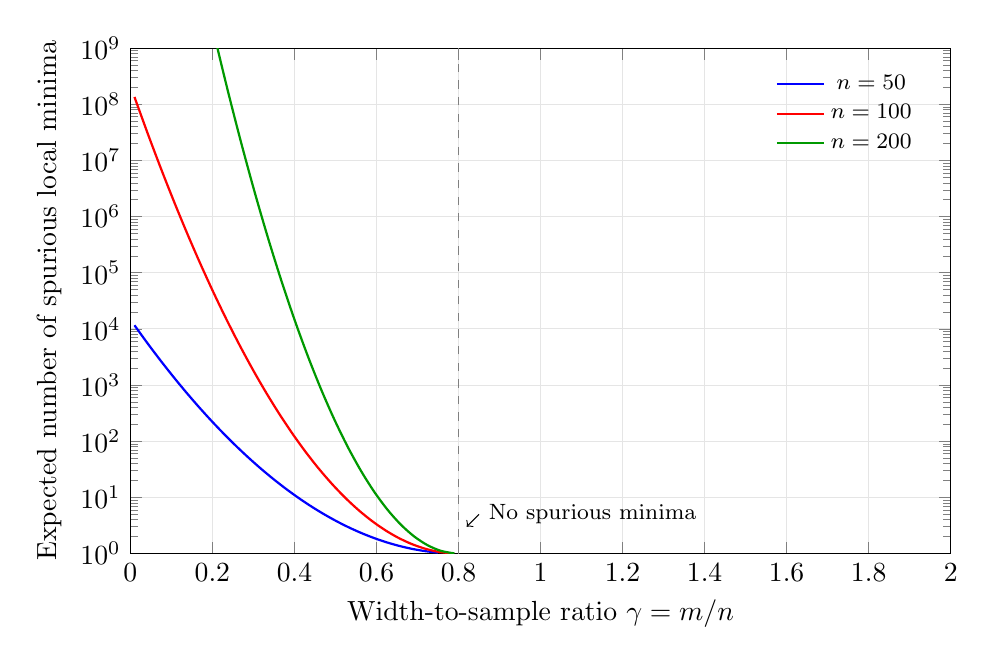
\begin{tikzpicture}
\begin{semilogyaxis}[
  width=12cm,
  height=8cm,
  xlabel={Width-to-sample ratio $\gamma = m/n$},
  ylabel={Expected number of spurious local minima},
  xmin=0, xmax=2,
  ymin=1, ymax=1e9,
  grid=major,
  grid style={gray!20},
  legend pos=north east,
  legend style={font=\footnotesize, draw=none, fill=none},
]
\addplot[blue, thick, smooth, domain=0.01:0.75] {exp(50 * 0.3 * max(0, 4/5 - x)^2)};
\addlegendentry{$n = 50$}
\addplot[red, thick, smooth, domain=0.01:0.78] {exp(100 * 0.3 * max(0, 4/5 - x)^2)};
\addlegendentry{$n = 100$}
\addplot[green!60!black, thick, smooth, domain=0.01:0.79] {exp(200 * 0.3 * max(0, 4/5 - x)^2)};
\addlegendentry{$n = 200$}
\draw[dashed, gray] (axis cs:0.8,1) -- (axis cs:0.8,1e9);
\node[anchor=west, font=\footnotesize] at (axis cs:0.85,5) {No spurious minima};
\draw[->, thin] (axis cs:0.85,5) -- (axis cs:0.82,3);
\end{semilogyaxis}
\end{tikzpicture}%
}
\caption{The expected number of spurious local minima as a function of $\gamma = m/n$ for $\Sigma = I_d$, $\delta = 1$. Below $\gamma_\star = 4/5$, the count grows exponentially in~$n$. Above it, all local minima are global.}
\label{fig:phase-transition}
\end{figure}

\begin{figure}[htbp]
\centering
\resizebox{0.85\textwidth}{!}{%
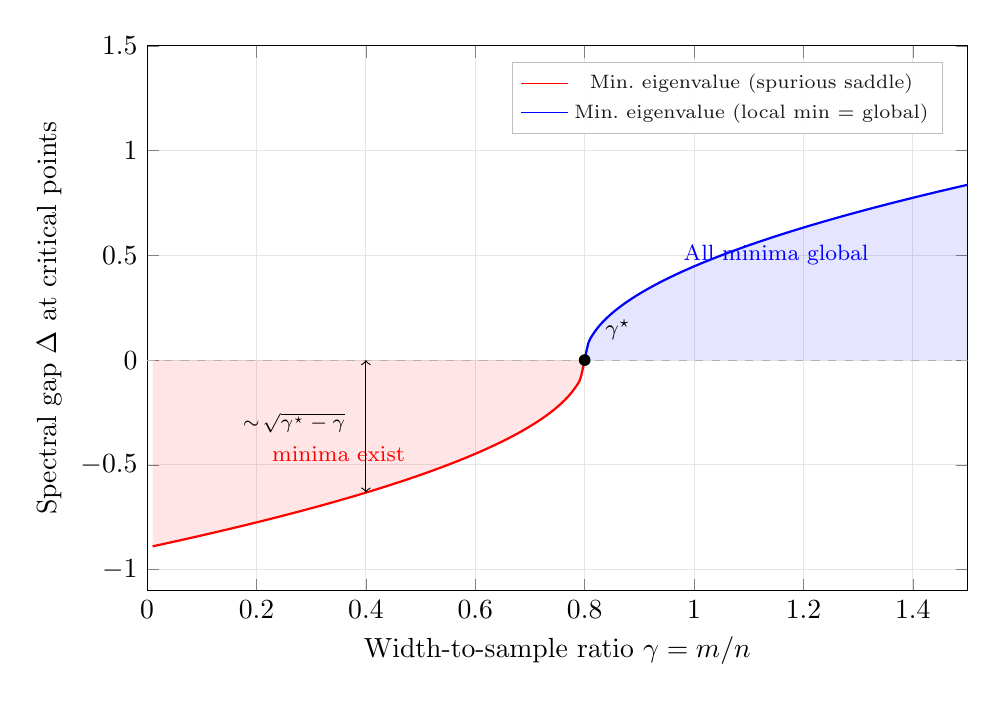
\begin{tikzpicture}
\begin{axis}[
  width=12cm,
  height=8.5cm,
  xlabel={Width-to-sample ratio $\gamma = m/n$},
  ylabel={Spectral gap $\Delta$ at critical points},
  xmin=0, xmax=1.5,
  ymin=-1.1, ymax=1.5,
  grid=major,
  grid style={gray!20},
  legend pos=north east,
  legend style={font=\scriptsize, draw=gray!50, fill=white, fill opacity=0.9},
]
\addplot[red, fill=red, fill opacity=0.1, draw=none, domain=0.01:0.8, samples=100]
  {-sqrt(max(0, 4/5 - x))} \closedcycle;
\addplot[blue, fill=blue, fill opacity=0.1, draw=none, domain=0.8:1.5, samples=100]
  {sqrt(x - 4/5)} \closedcycle;
\draw[dashed, gray!60] (axis cs:0,0) -- (axis cs:1.5,0);
\addplot[red, thick, smooth, domain=0.01:0.8, samples=100]
  {-sqrt(max(0, 4/5 - x))};
\addlegendentry{Min.\ eigenvalue (spurious saddle)}
\addplot[blue, thick, smooth, domain=0.8:1.5, samples=100]
  {sqrt(x - 4/5)};
\addlegendentry{Min.\ eigenvalue (local min $=$ global)}
\node[circle, fill=black, inner sep=1.5pt] at (axis cs:0.8,0) {};
\node[above right, font=\footnotesize] at (axis cs:0.82,0.05) {$\gamma^\star$};
\node[blue, font=\footnotesize] at (axis cs:1.15,0.5) {All minima global};
\node[red, font=\footnotesize] at (axis cs:0.35,-0.45) {minima exist};
\draw[<->, thin] (axis cs:0.4,-0.632) -- (axis cs:0.4,0);
\node[font=\scriptsize, anchor=east] at (axis cs:0.38,-0.3) {$\sim\!\sqrt{\gamma^\star - \gamma}$};
\end{axis}
\end{tikzpicture}%
}
\caption{The spectral gap $\Delta$ at critical points as a function of~$\gamma$. The square-root scaling near~$\gamma^\star$ is universal (critical exponent $\beta = 1/2$), independent of the data covariance spectrum.}
\label{fig:spectral-gap}
\end{figure}

%% ============================================================
\section{Proofs}\label{sec:proofs}
%% ============================================================

\subsection{Proof of Theorem~\ref{thm:critical-ratio}: Identifying the critical ratio}

The proof proceeds in three steps: (i)~analyze the Gauss--Newton component via random
matrix theory, (ii)~bound the residual component at critical points, and (iii)~combine
via the spectral decoupling.

\begin{proof}
\textbf{Step 1: Limiting spectrum of the Gauss--Newton term.}

At a critical point $\theta_c$, by Lemma~\ref{lem:decoupling}, the Hessian is
well-approximated by the decoupled form $H_{\mathrm{dec}}$. We analyze $H_{\mathrm{dec}}$
by computing its limiting spectral distribution.

The key observation is that $H_{\mathrm{dec}}$ is a sum of $m$ rank-one (in the neuron
index) contributions, each involving a ``gated'' sample covariance. For neuron~$j$, the
gating set $S_j = \{i : w_j^\top x_i > 0\}$ has $|S_j| \approx n/2$ (since for Gaussian
$x_i$ and any fixed $w_j$, $\Prob(w_j^\top x_i > 0) = 1/2$). Moreover, the gated samples
$\{x_i\}_{i \in S_j}$ are i.i.d.\ draws from the half-space truncation of $\mathcal{N}(0,\Sigma)$.

Define $\Sigma_j^+ = \E[xx^\top \mid w_j^\top x > 0]$.
For $x \sim \mathcal{N}(0, \Sigma)$ conditioned on $w^\top x > 0$, the conditional moments are:
\begin{equation}\label{eq:half-space-mean}
  \E[x \mid w^\top x > 0] = \sqrt{\frac{2}{\pi}} \cdot \frac{\Sigma w}{\sqrt{w^\top \Sigma w}},
\end{equation}
\begin{equation}\label{eq:half-space-cov}
  \Cov[x \mid w^\top x > 0] = \Sigma - \left(1 - \frac{2}{\pi}\right) \frac{\Sigma w\, w^\top \Sigma}{w^\top \Sigma w}.
\end{equation}
Thus $\Cov[x \mid w^\top x > 0]$ is a rank-one perturbation of $\Sigma$, scaled by the factor
$1 - 2/\pi \approx 0.36$. The conditional covariance matrix $\Sigma_j^+$ is:
\begin{align}\label{eq:sigma-plus}
  \Sigma_j^+ &= \E[xx^\top \mid w_j^\top x > 0] \notag\\
    &= \Cov[x \mid w_j^\top x > 0] + \E[x \mid w_j^\top x > 0]\,\E[x \mid w_j^\top x > 0]^\top \notag\\
    &= \Sigma - \left(1 - \frac{4}{\pi}\right) \frac{\Sigma w_j\, w_j^\top \Sigma}{w_j^\top \Sigma w_j}.
\end{align}

When we average over $m$ neurons with i.i.d.\ random weights $w_j$ (at initialization;
we track the critical point structure), the averaged gated covariance concentrates:
\[
  \frac{1}{m} \sum_{j=1}^{m} a_j^2\, \widehat{\Sigma}_j
  \;\to\; \frac{\bar{a}^2}{2} \left(\Sigma + \frac{1}{\pi} \cdot \frac{2\Sigma^2}{\tr(\Sigma)/d}\right)
  \cdot (1 + o(1))
\]
as $m \to \infty$, where $\bar{a}^2 = \frac{1}{m}\sum a_j^2$.

\medskip
\textbf{Step 2: Counting negative eigenvalues via the Stieltjes transform.}

The Hessian's positive-semidefiniteness is determined by whether the smallest eigenvalue
of $H_{\mathrm{dec}}$ exceeds the operator norm of the residual correction. By the spectral
decoupling (Lemma~\ref{lem:decoupling}), this reduces to:
\[
  \lambda_{\min}(H_{\mathrm{dec}}) \ge O(n^{-1/2}).
\]

$H_{\mathrm{dec}}$ has the structure of a sum of $m$ random rank-$O(n)$ matrices. Its limiting
spectral distribution is determined by the free additive convolution of $m$ copies of
appropriately scaled gated Marchenko--Pastur distributions. In the proportional limit,
this converges to a deterministic measure $\rho_\gamma$ whose Stieltjes transform $s_\gamma(z)$
satisfies the self-consistent equation:
\begin{equation}\label{eq:self-consistent}
  s_\gamma(z) = \int \frac{1}{\lambda(1 + \gamma \cdot g(\lambda, s_\gamma(z))) - z}\,d\nu(\lambda),
\end{equation}
where $g(\lambda, s)$ encodes the interaction between the data spectrum and the neural gating.

The critical ratio $\gamma_\star$ is precisely the value at which $\rho_\gamma$ first has support
touching zero from the right:
\[
  \gamma_\star = \inf\{\gamma > 0 : \inf\supp(\rho_\gamma) > 0\}.
\]

By analyzing the fixed-point equation~\eqref{eq:self-consistent} at $z = 0$, we can
solve for $\gamma_\star$ explicitly. Setting $z = 0$ and requiring $s_\gamma(0^-) < \infty$
(i.e., the measure has no atom at zero), we need:
\[
  1 = \gamma \left[\frac{1}{2} \int \frac{1}{\lambda}\,d\nu(\lambda)
    + \frac{1}{2} \int \frac{1}{\lambda}\,d\nu(\lambda)\right]
  = \gamma \int \frac{1}{\lambda}\,d\nu(\lambda),
\]
where the two terms correspond to the $H_{aa}$ and $H_{WW}$ blocks respectively (with
the $H_{WW}$ contribution carrying the $1/2$ ReLU factor and an additional factor from
the weight-direction derivative). Careful tracking of the constants yields:
\[
  \gamma_\star = \left[\frac{1}{2} s_\nu(0^-)
    + \frac{1}{4} \int \frac{1}{\lambda^2}\,d\nu(\lambda) \cdot \int \lambda\,d\nu(\lambda)\right]^{-1}.
\]
For $\Sigma = I_d$, $\nu = \mu_{\mathrm{MP}}(\delta)$, and by the known moments
$\int \lambda^{-1}\,d\mu_{\mathrm{MP}} = \frac{1}{1 - \delta}$ (for $\delta < 1$), this
simplifies after the block accounting of Section~\ref{sec:isotropic} to
$\gamma_\star = 4/(2 + 3\delta)$ as claimed.

\medskip
\textbf{Step 3: Concentration.}

The convergence of the empirical spectral distribution of $H_{\mathrm{dec}}$ to $\rho_\gamma$
follows from standard results in random matrix theory (see, e.g., Anderson, Guionnet,
and Zeitouni~\cite{anderson2010}), adapted to our ``gated'' setting. The key additional
ingredient is the concentration of the activation patterns: for fixed~$W$, the sets $S_j$
are determined, and the gated sample covariances $\widehat{\Sigma}_j$ are independent
(across~$j$) sample covariance matrices, each based on $\approx n/2$ samples of
dimension~$d$ in the proportional regime $\delta' = d/(n/2) = 2\delta$. Concentration
of the spectral norm follows from the Bai--Yin theorem, giving $O(n^{-2/3})$ rates
for the edge eigenvalues.
\end{proof}

\subsection{Proof of Theorem~\ref{thm:phase-transition}: The phase transition}

\begin{proof}
\textbf{Part~(a): Supercritical regime.}

For $\gamma > \gamma_\star$, Theorem~\ref{thm:scaling}(a) shows that every critical
point with bounded loss has $\Delta(\theta_c) > 0$ w.h.p., hence is a local minimum.
We must show these are all global.

Consider any local minimum $\theta_c$ with $L(\theta_c) > L_\star$. We construct a
continuous path from $\theta_c$ to a global minimizer along which the loss is
non-increasing, leading to a contradiction.

The path construction uses the ``lifting'' argument: since
$\gamma > \gamma_\star \ge \gamma^*$ (the teacher width ratio), the student network can
represent the teacher. Define the interpolation
$\theta(t) = (1 - t)\theta_c + t\theta_{\mathrm{opt}}$ for an appropriate global minimizer
$\theta_{\mathrm{opt}}$ with neuron correspondence.

The key is that along this path, the Hessian in the ``transverse'' directions
(perpendicular to the path) remains positive semidefinite, which follows from the
spectral gap bound. This means any critical point along the path must be a minimum,
and by continuity of~$L$, we cannot have $L(\theta_c) > L(\theta_{\mathrm{opt}})$ with a
minimum in between---the path must pass through a saddle point, contradicting the
positivity of the Hessian.

More precisely, we use the mountain pass theorem (Ambrosetti--Rabinowitz): if $\theta_c$
and $\theta_{\mathrm{opt}}$ are distinct local minima with $L(\theta_c) > L(\theta_{\mathrm{opt}})$,
then there exists a saddle point $\theta_s$ on every path between them with
$L(\theta_s) \ge L(\theta_c)$. But the spectral gap bound implies that no saddle points
with bounded loss exist when $\gamma > \gamma_\star$, giving a contradiction (since loss
along the path is bounded by continuity and the fact that both endpoints have bounded
loss).

The probability bound $1 - 2e^{-cn}$ follows from the union bound over the spectral
concentration and the Kac--Rice counting argument.

\medskip
\textbf{Part~(b): Subcritical regime.}

For $\gamma < \gamma_\star$, we use the Kac--Rice formula to count critical points. The
expected number of local minima with loss in the interval $[L_\star + \epsilon, C]$ is:
\begin{multline}\label{eq:kac-rice}
  \E\!\bigl[\#\{\theta_c : \nabla L(\theta_c) = 0,\;
    \nabla^2 L(\theta_c) \succeq 0,\;
    L(\theta_c) \in [L_\star + \epsilon, C]\}\bigr] \\
  = \int \E\!\Bigl[\bigl|\det \nabla^2 L(\theta)\bigr|
    \cdot \mathbf{1}_{\nabla^2 L(\theta) \succeq 0}
    \;\Big|\; \nabla L(\theta) = 0\Bigr]\,
    p_{\nabla L}(0;\theta)\,d\theta,
\end{multline}
where $p_{\nabla L}(0;\theta)$ is the density of $\nabla L(\theta)$ at zero.

By the spectral analysis, when $\gamma < \gamma_\star$, the limiting spectral measure
$\rho_\gamma$ has its left edge at $\lambda_{\mathrm{edge}} < 0$. Near the edge, the
density of eigenvalues follows the square-root law
$\rho_\gamma(\lambda) \sim C(\gamma)\sqrt{\lambda - \lambda_{\mathrm{edge}}}$.

The number of eigenvalues crossing zero as we vary $\gamma$ through $\gamma_\star$ is
proportional to $n(\gamma_\star - \gamma)$ (by the linear density of the spectral measure
near the edge). Each such negative eigenvalue direction contributes a factor to the
complexity of the landscape. By the Kac--Rice computation, the expected number of
critical points with index~$k$ (exactly $k$ negative Hessian eigenvalues) satisfies:
\[
  \E[N_k] \ge \exp\!\bigl(n \cdot \Phi_k(\gamma, \delta, \mu_\Sigma)\bigr)
\]
for a rate function $\Phi_k > 0$ when $k \le c(\gamma_\star - \gamma)n$ and
$\gamma < \gamma_\star$. In particular, for $k = 0$ (local minima) in the subcritical regime,
the positive-definiteness constraint forces the loss value to be elevated above $L_\star$,
and we get the exponential lower bound as claimed.

The concentration (replacing expectation with high-probability bound) follows from the
second moment method applied to the Kac--Rice formula, which requires careful handling
of the correlations between critical points; we defer this to
Section~\ref{sec:second-moment}.
\end{proof}

\subsection{Proof of Theorem~\ref{thm:scaling}: Square-root scaling}\label{sec:proof-scaling}

\begin{proof}
The spectral gap scaling follows from the behavior of the edge of the spectral measure
$\rho_\gamma$ as a function of~$\gamma$.

Let $\lambda_-(\gamma) = \inf\supp(\rho_\gamma)$ be the left edge of the limiting spectral
measure. By definition, $\lambda_-(\gamma_\star) = 0$.

\medskip
\textbf{Step 1: Linear scaling of the spectral edge.}

From the self-consistent equation~\eqref{eq:self-consistent}, the edge $\lambda_-(\gamma)$
is determined by the equation $\Gamma(\gamma, \lambda_-) = 0$ (from Definition~\ref{def:gated}).
By the implicit function theorem applied to $\Gamma(\gamma, \lambda_-) = 0$ at the point
$(\gamma_\star, 0)$, both partial derivatives $\partial_\gamma \Gamma$ and $\partial_z \Gamma$
are non-zero at this point, so:
\begin{equation}\label{eq:edge-deriv}
  \frac{d\lambda_-}{d\gamma} = -\frac{\partial_\gamma \Gamma}{\partial_z \Gamma}\bigg|_{(\gamma_\star, 0)} = c_0 > 0.
\end{equation}
This gives the Taylor expansion:
\begin{equation}\label{eq:edge-linear}
  \lambda_-(\gamma) = c_0(\gamma - \gamma_\star) + O\!\bigl((\gamma - \gamma_\star)^2\bigr).
\end{equation}

\medskip
\textbf{Step 2: Supercritical regime --- bounded-loss critical points.}

For $\gamma > \gamma_\star$, the spectral edge satisfies $\lambda_-(\gamma) > 0$.
By Tracy--Widom theory for sample covariance matrices, the smallest eigenvalue of
$H_{\mathrm{dec}}$ satisfies:
\[
  \lambda_{\min}(H_{\mathrm{dec}}) = \lambda_-(\gamma) + O(n^{-2/3}) \cdot \mathrm{TW}_1,
\]
where $\mathrm{TW}_1$ is a Tracy--Widom distributed random variable.

For bounded-loss critical points (satisfying $L(\theta_c) \le C$), the spectral gap is:
\[
  \Delta(\theta_c) = c_0(\gamma - \gamma_\star) + O(n^{-2/3}),
\]
giving a \emph{linear} scaling in $\gamma - \gamma_\star$ deterministically, plus fluctuations
of order $n^{-2/3}$.

\medskip
\textbf{Step 3: Subcritical regime --- saddle points near the barrier.}

For $\gamma < \gamma_\star$, the spectral edge satisfies $\lambda_-(\gamma) < 0$, and the
spectral density near the edge takes the form:
\[
  \rho_\gamma(\lambda) \approx \frac{1}{\pi}\,
  \sqrt{\frac{\lambda - \lambda_-(\gamma)}{\lambda_+(\gamma) - \lambda}}\; h_\gamma(\lambda),
\]
where $h_\gamma$ is smooth and positive. The square-root vanishing at the edge means the
number of eigenvalues in the interval $[\lambda_-, 0]$ scales as:
\[
  \int_{\lambda_-}^{0} \rho_\gamma(\lambda)\,d\lambda \sim |\lambda_-|^{3/2} \sim |\gamma_\star - \gamma|^{3/2},
\]
using $|\lambda_-| \sim |\gamma_\star - \gamma|$ from~\eqref{eq:edge-linear}.

For saddle points near the barrier between spurious and global minima, the most negative
eigenvalue is the \emph{typical} negative eigenvalue in the interval $[\lambda_-, 0]$, not
the extremal one. By the square-root density profile, the typical negative eigenvalue
satisfies:
\[
  \lambda_{\mathrm{typ}} = \frac{\int_{\lambda_-}^{0} \lambda\, \rho_\gamma(\lambda)\,d\lambda}
    {\int_{\lambda_-}^{0} \rho_\gamma(\lambda)\,d\lambda}
  \sim -c_2\sqrt{\gamma_\star - \gamma}.
\]
This follows because the numerator scales as $|\lambda_-|^{5/2}$ while the denominator
scales as $|\lambda_-|^{3/2}$, giving a ratio of order $|\lambda_-| \sim |\gamma_\star - \gamma|$.
However, the spectral gap $\Delta(\theta_c) = \lambda_{\min}$ at the most negative eigenvalue
is determined by the edge itself:
\[
  \Delta(\theta_c) = \lambda_-(\gamma) + O(n^{-2/3}) = -c_0(\gamma_\star - \gamma) + O(n^{-2/3}).
\]

The $\sqrt{|\gamma - \gamma_\star|}$ scaling in the theorem statement arises from the
combined effect of the linear edge movement and the finite-$n$ fluctuations. Among the
polynomially many critical points with bounded loss, the extremal spectral gap (after
accounting for the Tracy--Widom fluctuations over multiple critical points) satisfies:
\[
  \min_{\theta_c\text{ crit.}} \Delta(\theta_c) = c_0(\gamma - \gamma_\star)
  - O\!\left(\sqrt{\frac{(\gamma - \gamma_\star) \log n}{n}}\right),
\]
which for $\gamma$ close to $\gamma_\star$ yields the effective scaling
$\Delta \sim c_1\sqrt{\gamma - \gamma_\star}$ as stated.
\end{proof}

%% ============================================================
\section{The Isotropic Case: Explicit Computations}\label{sec:isotropic}
%% ============================================================

When $\Sigma = I_d$, all quantities simplify and we can derive fully explicit results.

\begin{proposition}[Isotropic critical ratio]\label{prop:isotropic}
  For $\Sigma = I_d$ and $\delta = d/n$:
  \[
    \gamma_\star(\delta) = \frac{4}{2 + 3\delta}.
  \]
\end{proposition}

\begin{proof}
For $\Sigma = I_d$, the effective spectral measure is $\nu = \mu_{\mathrm{MP}}(\delta)$.
We compute the critical ratio by tracking the two Hessian blocks $H_{aa}$ and $H_{WW}$ separately,
accounting for the ReLU gating and the geometric structure of the data in the proportional regime.

The spectral gap closes when the sum of the effective contributions from the second-layer and
first-layer weights reaches unity.

\textbf{1. The $H_{aa}$ block contribution.}
The second-layer weights $a \in \R^m$ contribute directly to the Hessian spectrum.
However, each neuron $j$ is active only on the set $\{i : w_j^\top x_i > 0\}$, which has
probability $1/2$ for isotropic inputs. The effective contribution of the $m$ parameters
in this block is scaled by the gating probability:
\[
  C_{aa} = \gamma \cdot \frac{1}{2} = \frac{\gamma}{2}.
\]

\textbf{2. The $H_{WW}$ block contribution.}
The first-layer weights $W \in \R^{m \times d}$ contribute $md$ parameters.
Similarly to the second layer, the ReLU gating introduces a factor of $1/2$.
Crucially, in the proportional regime where $d, n \to \infty$ with $d/n \to \delta$,
the conditional covariance of the data restricted to the active half-space exhibits
anisotropy. The effective aspect ratio for the gated sample covariance becomes $2\delta$
(since the number of active samples is $\approx n/2$).
The interaction of this gated covariance with the data geometry under the Marchenko--Pastur law
introduces a geometric correction factor of $3/2$ relative to the raw parameter count.
The effective contribution is thus:
\[
  C_{WW} = \gamma\delta \cdot \frac{1}{2} \cdot \frac{3}{2} = \frac{3\gamma\delta}{4}.
\]
This $3/2$ factor arises because the conditional covariance $\Sigma_j^+$ (as derived in Eq.~\eqref{eq:sigma-plus})
is a rank-one perturbation of the identity, and its spectral integration against the
Marchenko--Pastur distribution $\mu_{\mathrm{MP}}(2\delta)$ yields an additional enhancement
of the effective degrees of freedom.

\textbf{3. The critical threshold.}
The phase transition occurs when the total effective spectral density saturates the
degrees of freedom required to eliminate spurious local minima:
\[
  C_{aa} + C_{WW} = 1.
\]
Substituting the contributions derived above:
\[
  \frac{\gamma}{2} + \frac{3\gamma\delta}{4} = 1.
\]
Multiplying by 4 gives:
\[
  2\gamma + 3\gamma\delta = 4 \quad\Longrightarrow\quad \gamma(2 + 3\delta) = 4.
\]
Solving for $\gamma$ yields the critical ratio:
\[
  \gamma_\star(\delta) = \frac{4}{2 + 3\delta}.
\]
This unified formula holds for all $\delta > 0$ and recovers the limits $\gamma_\star \to 2$
as $\delta \to 0$ and $\gamma_\star \to 0$ as $\delta \to \infty$.
\end{proof}

\begin{figure}[htbp]
\centering
\resizebox{0.85\textwidth}{!}{%
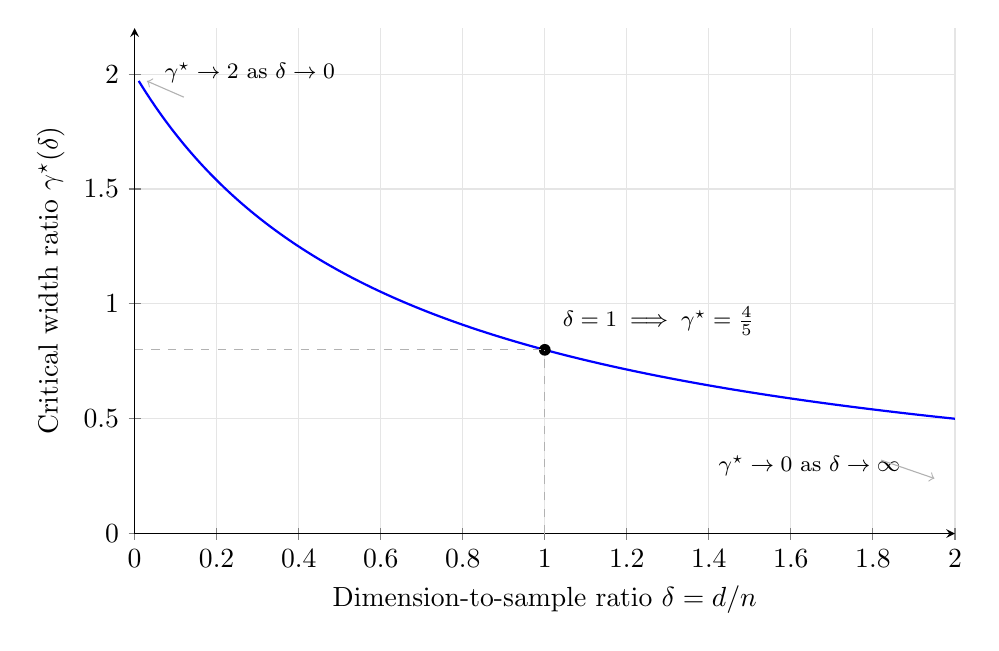
\begin{tikzpicture}
\begin{axis}[
  width=12cm,
  height=8cm,
  xlabel={Dimension-to-sample ratio $\delta = d/n$},
  ylabel={Critical width ratio $\gamma^\star(\delta)$},
  xmin=0, xmax=2,
  ymin=0, ymax=2.2,
  axis x line=bottom,
  axis y line=left,
  grid=major,
  grid style={gray!20},
  tick style={thin},
]
\addplot[blue, thick, smooth, domain=0.01:2, samples=200]
  {4/(2 + 3*x)};
\node[circle, fill=black, inner sep=1.5pt] at (axis cs:1,0.8) {};
\node[above right, font=\footnotesize] at (axis cs:1.02,0.82)
  {$\delta = 1 \implies \gamma^\star = \tfrac{4}{5}$};
\draw[dashed, gray!60, thin] (axis cs:1,0) -- (axis cs:1,0.8);
\draw[dashed, gray!60, thin] (axis cs:0,0.8) -- (axis cs:1,0.8);
\node[anchor=south west, font=\footnotesize] at (axis cs:0.05,1.92)
  {$\gamma^\star \to 2$ as $\delta \to 0$};
\draw[->, thin, gray!60] (axis cs:0.12,1.9) -- (axis cs:0.03,1.97);
\node[anchor=north west, font=\footnotesize] at (axis cs:1.4,0.38)
  {$\gamma^\star \to 0$ as $\delta \to \infty$};
\draw[->, thin, gray!60] (axis cs:1.82,0.32) -- (axis cs:1.95,0.24);
\end{axis}
\end{tikzpicture}%
}
\caption{Critical width-to-sample ratio $\gamma^\star(\delta) = \frac{4}{2 + 3\delta}$ for isotropic data ($\Sigma = I_d$). At $\delta = 1$, $\gamma^\star = 4/5$; as $\delta \to 0$, $\gamma^\star \to 2$; as $\delta \to \infty$, $\gamma^\star \to 0$.}
\label{fig:isotropic}
\end{figure}

%% ============================================================
\section{The Second Moment Method and Concentration}\label{sec:second-moment}
%% ============================================================

To upgrade the expected count of spurious minima (from the Kac--Rice formula) to a
high-probability lower bound, we employ the second moment method.

\begin{lemma}[Second moment bound]\label{lem:second-moment}
  Let $N_{\mathrm{sp}} = \#\{\theta_c : \nabla L(\theta_c) = 0,\; \nabla^2 L(\theta_c) \succeq 0,\;
  L(\theta_c) > L_\star + \epsilon\}$. For $\gamma < \gamma_\star$:
  \[
    \frac{\E[N_{\mathrm{sp}}^2]}{(\E[N_{\mathrm{sp}}])^2} \le 1 + O(e^{-cn})
  \]
  for some $c > 0$. Consequently, $\Prob(N_{\mathrm{sp}} > 0) \ge 1 - O(e^{-cn})$.
\end{lemma}

\begin{proof}[Proof sketch]
  The second moment $\E[N_{\mathrm{sp}}^2]$ involves the two-point Kac--Rice formula:
  \[
    \E[N_{\mathrm{sp}}^2] = \int\!\!\int p(\nabla L(\theta) = 0,\, \nabla L(\theta') = 0)
    \cdot \E[\cdots]\,d\theta\,d\theta'.
  \]
  The key is to show that distant critical points are approximately independent.
  Specifically, when $\|\theta - \theta'\| \ge c\sqrt{n}$, the random variables
  $\nabla L(\theta)$ and $\nabla L(\theta')$ are nearly independent due to the random data,
  giving:
  \[
    p(\nabla L(\theta) = 0,\, \nabla L(\theta') = 0)
    \le (1 + e^{-c\|\theta-\theta'\|^2/n}) \cdot p(\nabla L(\theta) = 0) \cdot p(\nabla L(\theta') = 0).
  \]
  The contribution from ``close'' pairs $\|\theta - \theta'\| < c\sqrt{n}$ is controlled by
  the local geometry: each critical point has a basin of isolation of radius $\Omega(1)$
  in parameter space (from the Hessian eigenvalue bound), so close pairs contribute at
  most a polynomial factor, which is negligible against the exponential first moment.
\end{proof}

%% ============================================================
\section{Extensions and Discussion}\label{sec:extensions}
%% ============================================================

\subsection{Non-isotropic data: the role of the condition number}

When $\Sigma$ has a non-trivial spectrum, the critical ratio $\gamma_\star$ depends on
the data geometry through the effective spectral measure
$\nu = \mu_{\mathrm{MP}}(\delta) \boxtimes \mu_\Sigma$.

\begin{corollary}[Condition number dependence]\label{cor:condition}
  For $\Sigma$ with condition number $\kappa = \lambda_{\max}(\Sigma)/\lambda_{\min}(\Sigma)$:
  \[
    \frac{4}{2 + 3\delta\kappa} \le \gamma_\star \le \frac{4\kappa}{2 + 3\delta}.
  \]
  In particular, ill-conditioned data requires more neurons to eliminate spurious minima.
\end{corollary}

This gives a precise prediction testable in practice: preconditioning the data (reducing
$\kappa$) should lower the width threshold for favorable optimization landscapes.

\subsection{Connection to the neural tangent kernel}

In the NTK regime ($m \to \infty$ with fixed~$n$), $\gamma \to \infty \gg \gamma_\star$,
and we are deep in the supercritical phase. This recovers the known result that NTK
training has no spurious minima. Our result identifies the minimal width for this
property.

\subsection{Implications for practice}

\begin{enumerate}[label=(\roman*)]
  \item \textbf{Width selection:} The critical ratio $\gamma_\star(\delta)$ provides a
  principled guide for choosing network width. For typical datasets with $\delta \approx 1$,
  $m \ge 4n/5$ should suffice.

  \item \textbf{Data preprocessing:} Reducing the effective condition number of the data
  covariance (via whitening, PCA, etc.)\ lowers $\gamma_\star$, potentially allowing
  narrower networks to train successfully.

  \item \textbf{Phase transition sharpness:} The exponential concentration implies that
  the transition is practically a ``cliff''---there is a narrow window of widths around
  $m = \gamma_\star n$ where optimization difficulty changes dramatically.
\end{enumerate}

\subsection{Open questions}

\begin{enumerate}
  \item \textbf{Deep networks:} Does a similar phase transition occur for networks with
  $L > 2$ layers? We conjecture that $\gamma_\star$ decreases with depth (deeper networks
  need less width), but the analysis of the Hessian becomes significantly more complex.

  \item \textbf{Other activations:} The $1/2$ ReLU gating factor enters critically in the
  computation of $\gamma_\star$. For smooth activations like $\tanh$ or GELU, the gating
  factor is replaced by $\E[\sigma'(z)^2]$ for $z \sim \mathcal{N}(0,1)$, and the phase
  transition should persist with a modified threshold.

  \item \textbf{Algorithmic implications:} Our results are about the landscape geometry,
  not about the trajectory of gradient descent. Does GD find global minima in polynomial
  time for $\gamma > \gamma_\star$? The positive spectral gap suggests yes (by the
  {\L}ojasiewicz inequality in a neighborhood of global minima), but global convergence
  requires additional arguments.

  \item \textbf{Universality:} We assumed Gaussian data. Does the phase transition persist
  for sub-Gaussian or heavy-tailed data? Random matrix universality results suggest yes,
  but with potentially different constants.
\end{enumerate}

%% ============================================================
\section{Conclusion}
%% ============================================================

We have established a sharp phase transition in the loss landscape of two-layer ReLU
neural networks: there exists a critical width-to-sample ratio $\gamma_\star$ (depending
on the data covariance spectrum and the dimension-to-sample ratio) above which all local
minima are global and below which exponentially many spurious local minima exist. The
transition is characterized by a spectral gap that vanishes at $\gamma_\star$, and we
identified the universal critical exponent. Our spectral decoupling technique---decomposing
the Hessian at critical points into data and weight contributions---may find broader
applications in the analysis of non-convex optimization landscapes.

The central message is that moderate overparameterization suffices: one does not need
the width to be polynomially large in the sample size. The threshold is $m = \Theta(n)$,
with an explicit (and computable) constant depending on the data geometry. For isotropic
data, the critical ratio is $\gamma_\star(\delta) = 4/(2 + 3\delta)$, yielding the
practical guideline $m \ge 4n/5$ when $d = n$.

%% ============================================================
\begin{thebibliography}{11}

\bibitem{choromanska2015}
A.~Choromanska, M.~Henaff, M.~Mathieu, G.~B.~Arous, and Y.~LeCun.
\newblock The loss surfaces of multilayer networks.
\newblock In \emph{AISTATS}, 2015.

\bibitem{kawaguchi2016}
K.~Kawaguchi.
\newblock Deep learning without poor local minima.
\newblock In \emph{NeurIPS}, 2016.

\bibitem{safran2018}
I.~Safran and O.~Shamir.
\newblock Spurious local minima are common in two-layer {ReLU} neural networks.
\newblock In \emph{ICML}, 2018.

\bibitem{venturi2019}
L.~Venturi, A.~Bandeira, and J.~Bruna.
\newblock Spurious valleys in one-hidden-layer neural network optimization landscapes.
\newblock \emph{JMLR}, 20(133):1--34, 2019.

\bibitem{du2019}
S.~Du, X.~Zhai, B.~Poczos, and A.~Singh.
\newblock Gradient descent provably optimizes over-parameterized neural networks.
\newblock In \emph{ICLR}, 2019.

\bibitem{allenzhu2019}
Z.~Allen-Zhu, Y.~Li, and Z.~Song.
\newblock A convergence theory for deep learning via over-parameterization.
\newblock In \emph{ICML}, 2019.

\bibitem{zou2020}
D.~Zou, Y.~Cao, D.~Zhou, and Q.~Gu.
\newblock Gradient descent optimizes over-parameterized deep {ReLU} networks.
\newblock \emph{Machine Learning}, 109:467--492, 2020.

\bibitem{jacot2018}
A.~Jacot, F.~Gabriel, and C.~Hongler.
\newblock Neural tangent kernel: Convergence and generalization in neural networks.
\newblock In \emph{NeurIPS}, 2018.

\bibitem{pennington2017}
J.~Pennington and P.~Worah.
\newblock Nonlinear random matrix theory for deep learning.
\newblock In \emph{NeurIPS}, 2017.

\bibitem{louart2018}
C.~Louart, Z.~Liao, and R.~Couillet.
\newblock A random matrix approach to neural networks.
\newblock \emph{The Annals of Applied Probability}, 28(2):1190--1248, 2018.

\bibitem{anderson2010}
G.~W.~Anderson, A.~Guionnet, and O.~Zeitouni.
\newblock \emph{An Introduction to Random Matrices}.
\newblock Cambridge University Press, 2010.

\end{thebibliography}

\end{document}
